\section{RESULTADOS}


En los resultados se comunican los hallazgos y descubrimientos del estudio. Se incluyen tablas, figuras, diagramas y demás material demostrativo.

Al narrar descriptivamente una figura, tabla, etc., en un párrafo, puedes insertar una referencia cruzada, es decir, un hipervínculo al elemento mencionado dentro o fuera de paréntesis, ejemplos: estos resultados se muestran en la \textbf{Tabla \ref{table:prob_milenio}}.  Igualmente, los datos son validados con otros instrumentos \textbf{(Tabla \ref{table:num_mersenne}, Tabla \ref{table:medalla_fields})}. Lineamientos que se establecen en la nueva versión de las Normas APA séptima edición \textbf{(Fig. \ref{figportada_apa})}. La producción intelectual institucional se publica en el Repositorio \textbf{(Fig. \ref{fig:escudo_udea})}. Si la figura es de tu completa autoría, \textbf{NO} es necesario colocar la leyenda “Elaboración propia” \textbf{(Fig. \ref{fig:hiperbolica})}.

\begin{figure}[!ht]
    \begin{center}
    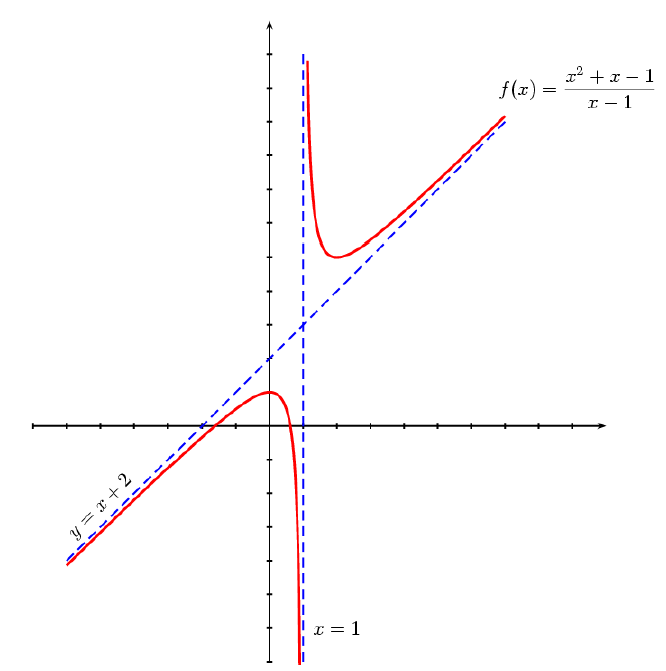
\includegraphics[scale=0.5]{imgs/grafica.png}\\
    \end{center}
    \caption{Función hiperbólica}
    \label{fig:hiperbolica}
    \textit{}
\end{figure}

\begin{table}%[!ht]
\caption{\MakeUppercase{Problemas del milenio: la resolucion de uno de estos problemas se premian con un monto de us\$ 1 millon}}
\begin{center}
\begin{tabular}{  l c }
    \hline
    1 & El problema de $P$ frente a $NP$  \\ \hline
    2 &  La conjetura de Hodge \\ \hline
    3 &  La conjetura de Poincaré \\ \hline
    4 &  La hipótesis de Riemann \\ \hline
    5 &  Yang-Mills y el salto de masa ("mass gap")\\ \hline
    6 &  Las ecuaciones de Navier-Stokes\\ \hline
    7 &  Conjetura de Birch y Swinnerton-Dyer\\
        \hline
\end{tabular}
\end{center}
\label{table:prob_milenio}
\end{table}

%\clearpage

\begin{table}%[!ht]
\caption{\MakeUppercase{Medalla Fields: matemáticos galardonados con este premio desde 2010; la medalla Fields se comenzó a entregar desde 1936}}
\begin{center}
\begin{tabular}{cp{4cm}p{2.5cm}p{6cm}}
    \hline
    año & Ganador(es) & pais & universidad/instituto\\
    \hline 
        2010 & Elon Lindenstrauss & Israel & Universidad Hebrea de Jerusalén\\
         & Ngo Bao Chau ,  & Vietnam y Francia &Paris-Sud 11 University y Institute for Advanced Study \\
         & Stanislav Smirnov  & Rusia & Universidad de Ginebra\\
         & Cédric Villani & Francia & Institut Henri Poincaré\\
         \hline
         2014 & Artur Ávila  & Francia &Instituto Nacional de Matemática Pura y Aplicada \\
         & Manjul Bhargava  &  Canadá y Estados Unidos &Universidad de Princeton \\
         & Martin Hairer & Austria & Imperial College London\\
         & Maryam Mirzajani & Irán &Universidad Stanford \\
         \hline\\
         2018	 & Caucher Birkar & Irán y Reino Unido & Universidad de Cambridge \\
         & Alessio Figalli & Italia & Escuela Politécnica Federal de Zúrich \\
         & Peter Scholze & Alemania & Universidad de Bonn\\
         & Akshay Venkatesh  & Australia & Universidad Stanford\\
        \hline
\end{tabular}
\end{center}
\label{table:medalla_fields}
\end{table}

\clearpage

\begin{table}%[!ht]
\caption{\MakeUppercase{Algunos números primos de Mersenne}}
\begin{center}
\begin{tabular}{ c|c}
    \hline
    Exponente $n$ & Primo de Mersenne \\ \hline
    2 &  $2^{2}-1=3 $ \\ \hline
    3 &  $2^{3}-1=7 $ \\ \hline
    5 &  $2^{5}-1=31 $ \\ \hline
    7 &  $2^{7}-1=127 $ \\ \hline
    13 &  $2^{13}-1=8191 $ \\ \hline
    17 &  $2^{17}-1=131071 $ \\
        \hline
\end{tabular}
\end{center}
\label{table:num_mersenne}
\end{table}


\begin{figure}[!ht]
    \begin{center}
    
\includegraphics[scale=0.5]{imgs/ieee_logo.jpg}\\
    \end{center}
    \caption{Imagen corporativa Institute of Electrical and Electronics Engineers (IEEE)}
    \label{figportada_apa}
    \footnotesize{Nota. Fuente \url{https://www.ieee.org/} Esta entidad edita y normaliza la presentación de documentos científicos en el área de ingenierías.} %\citep{lib:apa}.
\end{figure}

\clearpage

\begin{figure}[!ht]
    \begin{center}
    
\includegraphics{imgs/escudo_udea_solo.png}\\
    \end{center}
    \caption{Logo Universidad de Antioquia}
    \label{fig:escudo_udea}
    \footnotesize{Nota. Fuente \url{http:/www.udea.edu.co}}
\end{figure}

\clearpage